% \documentclass[dvipdfmx, 11pt]{beamer}
\documentclass[aspectratio=169, dvipdfmx, 11pt]{beamer} % aspectratio=43, 149, 169
\usepackage{here, amsmath, latexsym, amssymb, bm, ascmac, mathtools, multicol, tcolorbox, subfig}

%デザインの選択(省略可)
\usetheme{Luebeck}
%カラーテーマの選択(省略可)
\usecolortheme{orchid}
%フォントテーマの選択(省略可)
\usefonttheme{professionalfonts}
%フレーム内のテーマの選択(省略可)
\useinnertheme{circles}
%フレーム外側のテーマの選択(省略可)
\useoutertheme{infolines}
%しおりの文字化け解消
\usepackage{atbegshi}
\ifnum 42146=\euc"A4A2
\AtBeginShipoutFirst{\special{pdf:tounicode EUC-UCS2}}
\else
\AtBeginShipoutFirst{\special{pdf:tounicode 90ms-RKSJ-UCS2}}
\fi
%ナビゲーションバー非表示
\setbeamertemplate{navigation symbols}{}
%既定をゴシック体に
\renewcommand{\kanjifamilydefault}{\gtdefault}
%タイトル色
\setbeamercolor{title}{fg=structure, bg=}
%フレームタイトル色
\setbeamercolor{frametitle}{fg=structure, bg=}
%スライド番号のみ表示
%\setbeamertemplate{footline}[frame number]
%itemize
\setbeamertemplate{itemize item}{\small\raise0.5pt\hbox{$\bullet$}}
\setbeamertemplate{itemize subitem}{\tiny\raise1.5pt\hbox{$\blacktriangleright$}}
\setbeamertemplate{itemize subsubitem}{\tiny\raise1.5pt\hbox{$\bigstar$}}
% color
\newcommand{\red}[1]{\textcolor{red}{#1}}
\newcommand{\green}[1]{\textcolor{green!40!black}{#1}}
\newcommand{\blue}[1]{\textcolor{blue!80!black}{#1}}

%block_diagram
\usepackage{tikz}
\usetikzlibrary{calc}
\usetikzlibrary{positioning}
\usetikzlibrary{arrows.meta}

\title[Short title]{タイトル}
\subtitle{副題}
\author[著者略称]{氏名}
\institute[所属略称]{所属}
\date{\today}

\begin{document}
\maketitle

\begin{frame}{目次}
    \tableofcontents
\end{frame}

\begin{frame}{ブロック線図}
    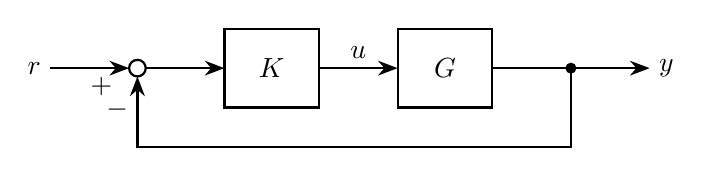
\begin{tikzpicture}
        [
        % 線と文字の間の間隔を設定
        every node/.style={outer sep=0.12cm, inner sep=0},
        % 矢印の設定
        arrow/.style={-{Stealth[length=0.25cm]}, thick},
        % ブロック
        block/.style={rectangle, draw, minimum height = 1cm,
        minimum width=1.2cm, thick, outer sep = 0},
        % 加え合わせ点
        sum/.style={thick, circle, draw, inner sep=0,
        minimum size=6pt, outer sep=0},
        % 引き出し点
        point/.style={radius=2pt}
        ]
        \node [block] (K){$K$};
        \node [block, right=1 of K] (G){$G$};
        \node [sum, left=1of K] (sum){};
        \draw[arrow] (sum) -- (K);
        \draw[arrow] (K) -- (G) node [above, pos=0.5] {$u$};
        \draw[arrow] (G.east) -- +(2, 0) node[right]{$y$};
        \draw[arrow] (sum.west)+(-1, 0) node[left]{$r$} -- (sum.west)
        node[below, xshift=-10pt]{$+$};
        \fill [point] (G.east)+(1, 0) circle coordinate (y);
        \draw [arrow] (y) -- +(0, -1) -| (sum) node[left, yshift=-15pt] {$-$};
    \end{tikzpicture}
\end{frame}

\end{document}